%cSpell:disable
\section{Datenanalyse}\label{sec:createportfolio}

%cSpell:disable
\subsection{Hypothekendaten}
In diesem Abschnitt wird der von der Münchener Hypothekenbank bereitgestellte Geschäftsbericht analysiert. Für die Prognose von Schäden an bestimmten Gebäuden wird ein Portfolio benötigt, das ein repräsentatives Bankportfolio darstellt. Da die vertraulichen Wohnimmobilien-Hypothekenportfolios von Banken nicht offengelegt werden, ist die Konstruktion eines annähernd realistischen Portfolios erforderlich. Es wird untersucht, welche Faktoren bei der Bestimmung von Größe und Zusammensetzung eines Wohnimmobilien-Hypothekenportfolios berücksichtigt werden. Darüber hinaus wird dargelegt, wie Daten zu Kreditmerkmalen, insbesondere Beleihungsquoten, in das Portfolio integriert werden.

Zum Stichtag 31.12.2023 belief sich der ausstehende Bestand an Wohnimmobilienfinanzierungen im Portfolio der \textcite{MuenchenerHyp2023} in Bayern auf 8.921.489.311,00 €, wobei die durchschnittliche Größe der Darlehen für Wohnimmobilien circa 163.700,00 € betrug. Zur Ermittlung der Anzahl der Darlehen im Portfolio wird zunächst der Gesamtbestand durch die durchschnittliche Größe der Darlehen dividiert, was gerundet 54.500 Darlehen ergibt. Unter Anwendung der Gleichung \ref{eq:cochran} zur Berechnung der erforderlichen Stichprobengröße für das theoretische Szenario einer unendlichen Anzahl von Immobilien im Portfolio ergibt sich bei einem Konfidenzintervall von 99\% und einer Fehlermarge von 2\% ein notwendiger Stichprobenumfang von 4.147 Datenpunkten. Die in Gleichung \ref{eq:finite_population} präsentierte Formulierung für endliche Populationen führt jedoch zu einer Reduktion auf 3.853 Darlehen als erforderliche Stichprobengröße für Portfolios mit 54.500 Elementen.

Neben der Anzahl der Darlehen ist auch deren Qualität, insbesondere der Beleihungsauslauf, von entscheidender Bedeutung für die Repräsentativität des Portfolios. Da die in den Geschäftsberichten ausgewiesenen Kreditbestände lediglich das Risikoexposure des Kreditinstituts reflektieren und nicht den realen Immobilienwert repräsentieren, ergibt sich die Notwendigkeit, den Property Value in Relation zum Gesamtrisikoexposure zu evaluieren. Die Münchener Hypothekenbank hat in ihrem Jahresbericht die Verteilung des Beleihungsauslaufs in tabellarischer Form offengelegt (siehe Tabelle \ref{tab:beleihungsauslauf2023}). Darüber hinaus wurde ein durchschnittlicher Beleihungsauslauf von 54,1\% für die Wohnimmobilienfinanzierung angegeben. Diese Informationen stellen die fundamentalen finanziellen Parameter dar, die für die Konstruktion eines repräsentativen Immobilienportfolios essenziell sind.

\begin{table}[htbp]
    \centering
    \caption{Verteilung des Beleihungsauslaufs im Wohnimmobilienportfolio der Münchener Hypothekenbank zum 31.12.2023}
    \label{tab:beleihungsauslauf2023}
    \small  % Slightly larger font than \footnotesize
    \begin{tabularx}{\textwidth}{>{\raggedright\arraybackslash}X*{6}{>{\centering\arraybackslash}X}} 
    \toprule
    \textbf{LtV} & $\leq 60\%$ & $60$--$70\%$ & $70$--$80\%$ & $80$--$90\%$ & $90$--$100\%$ & $>100\%$ \\
    \cmidrule(lr){1-7}  % Dòng kẻ mảnh hơn dưới tên các cột
    \textbf{Prozentanteil} & 39,2\% & 15,0\% & 16,4\% & 10,2\% & 8,2\% & 11,0\% \\
    \bottomrule
    \end{tabularx}
\end{table}
%cSpell:disable
\subsection{Geodaten zu Hypotheken und Hochwasser}
\subsubsection{Hypothekengeodaten}\label{sec:hypogeo}

Für die Kompatibilität von Hypotheken- und Hochwasserdaten sind geografische Koordinaten erforderlich. Dieser Abschnitt befasst sich mit der Generierung präziser Koordinaten für die Datenpunkte.

Eine zufällige Verteilung in Bayern würde die Struktur eines Kreditportfolios nicht korrekt abbilden, da eine ungleichmäßige Verteilung von Immobilien sowohl in Deutschland als auch in Bayern zu beobachten ist. \textcite{zurek2022real} analysierte die Beziehung zwischen Bevölkerungsdichte und Kreditvergabe in Deutschland. Die Studie zeigt, dass Regionen mit stärkerem Wirtschaftswachstum höhere Immobilienpreise aufweisen. Dies führt zu einer erhöhten Kreditnachfrage. Auf Basis dieser empirischen Erkenntnisse wird die Bevölkerungsdichte als Grundlage für die Zuweisung spezifischer Koordinaten zu jedem Datenpunkt herangezogen.

Die verwendete Datenquelle stammt von \textcite{suche_postleitzahl}. Sie kombiniert OpenStreetMap-Daten mit Einwohnerzahlen von \textcite{destatis}. Dies ermöglicht eine präzise Segmentierung in Postleitzahlenzonen. Tabelle \ref{tab:geodaten} zeigt die Daten dieser geographischen Strukturierung.
Übersicht der Geodaten für Postleitzahlgebiete in Bayern
\begin{table}[htbp]
    \centering
    \small
    \caption{Übersicht der Geodaten für Postleitzahlgebiete in Bayern}
    \label{tab:geodaten}
    \begin{tabularx}{1.0\textwidth}{>{\raggedright\arraybackslash}X >{\raggedright\arraybackslash}X}
        \toprule
        \textbf{Objekt} & \textbf{Erklärung} \\
        \midrule
        plz & Postleitzahl \\
        \addlinespace
        einwohner & Die Einwohnerzahl eines bestimmten Ortes \\
        \addlinespace
        qkm & Die Fläche des Gebiets in Quadratkilometern \\
        \addlinespace
        geometry & Die Koordinaten des Gebiets \\
        \addlinespace
        ort & Der Name des Ortes, in dem sich das Gebiet befindet \\
        \addlinespace
        landkreis & Die Zugehörigkeit zu einem Landkreis \\
        \bottomrule
    \end{tabularx}
\end{table}
\FloatBarrier


Tabelle \ref{tab:geodaten} wurde aus Shapefile-Daten der Postleitzahlenregionen generiert und umfasst die Bevölkerungsverteilung. Vier Spalten sind von besonderer Relevanz: Ort, Landkreis, Geometrie und Einwohner. Die Geometriespalte enthält die geografischen Koordinaten der Gemeinden, dargestellt als Polygon oder Multipolygon. Ein Multipolygon setzt sich aus mehreren Einzelpolygonen verschiedener Formen zusammen. Zur räumlichen Referenzierung dient das Koordinatensystem EPSG:3035. Abbildung \ref{fig:bevoelkerungsdichte} visualisiert die aus diesen Daten abgeleitete Bevölkerungsdichteverteilung Bayerns nach Postleitzahlenbereichen.

\begin{figure}[htbp]
    \centering
    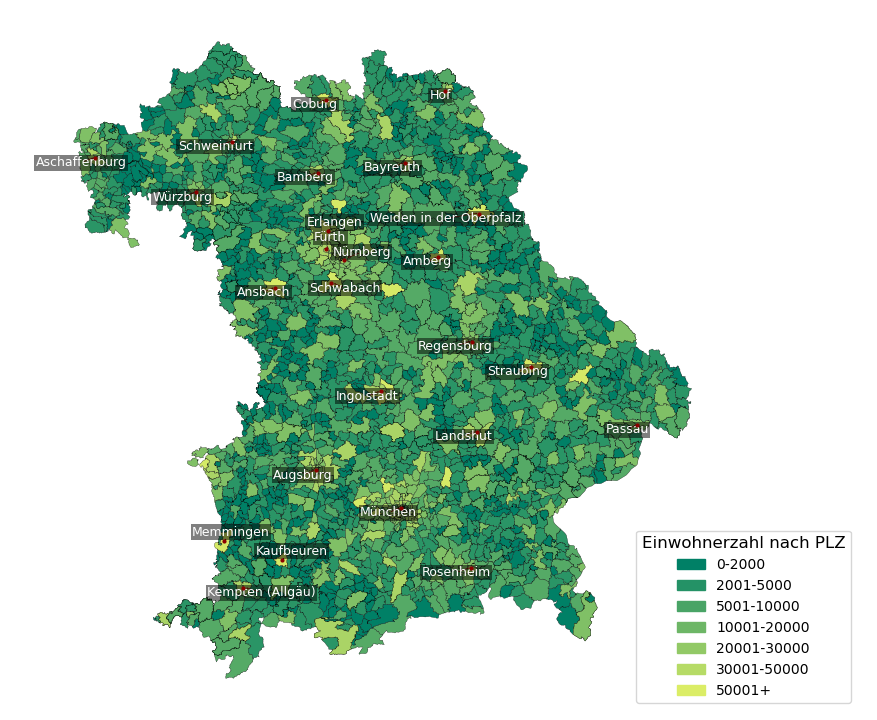
\includegraphics[width=0.95\textwidth]{figures/Bayern_pop_plz.png}
    \caption{Verteilung der Bevölkerungsdichte Bayerns nach Postleitzahlenbereichen. Quelle: Eigene Darstellung}
    \label{fig:bevoelkerungsdichte}
\end{figure}
\FloatBarrier



\subsubsection{Hochwassergeodaten}\label{sec:hochgeo}

Im Anschluss an die in Abschnitt \ref{sec:hypogeo} dargelegte Erfassung der geografischen Koordinaten der Hypothekendarlehen ergibt sich die Notwendigkeit einer weiterführenden Analyse. Diese zielt darauf ab, die räumliche Relation der betreffenden Immobilien zu den definierten Hochwasserrisikogebieten zu determinieren. Zur Durchführung dieser Analyse ist eine detaillierte Hochwasserrisikokarte für Bayern erforderlich.

Im Rahmen eines EU-weiten Stresstests stellt die \ac{EZB} den Banken zur Simulation eines schweren Überschwemmungsszenarios eine Hochwasserrisikokarte (Abbildung \ref{fig:euflut}) zur Verfügung.

\begin{figure}[htbp]
    \centering
    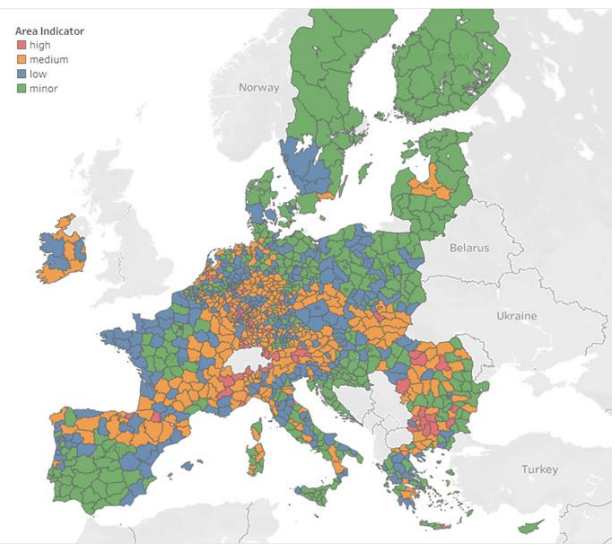
\includegraphics[width=0.6\textwidth]{figures/euflood.png} 
    \caption{EU-Hochwasserrisikokarte.Quelle: EZB 2022 Klimarisiko-Stresstest}
    \label{fig:euflut}
\end{figure}
\FloatBarrier

Die \ac{EZB}-Karte klassifiziert Regionen nach Hochwasserrisiken. Sie basiert auf Daten der Europäischen Kommission und Four Twenty Seven \parencite{ECB2022ClimateStressTest}. Allerdings sind die Basisdaten nicht öffentlich zugänglich. Zudem erlaubt die visuelle Darstellung keine präzise Identifikation spezifischer Gebiete. Folglich ergibt sich für Bayern die Notwendigkeit einer detaillierteren Analyse.

Die Kartierungen des Bayerischen Landesamts für Umwelt bieten eine fundierte Grundlage für die regionale Risikoanalyse. Diese für die Einzugsgebiete von Donau, Rhein und Elbe entwickelten Karten ermöglichen eine präzise Einschätzung der Hochwasserrisiken in Bayern \parencite{LfU_Bayern}. Sie visualisieren detailliert die Hochwassergefährdung, potenziell betroffene Landnutzungen und historische Hochwasserereignisse.
Diese Daten liegen im ETRS89-Koordinatensystem vor, während die Hypothekengeodaten das EPSG:3035-System nutzen. ETRS89 ist ein geodätisches Referenzsystem für Europa. Es misst Positionen in geografischen Koordinaten: Breitengrad und Längengrad. Diese werden in Grad, Minuten und Sekunden angegeben. ETRS89 bietet eine hohe Genauigkeit für kontinentale Messungen.
EPSG:3035 hingegen ist eine kartografische Projektion. Sie wandelt die Erdkrümmung in eine flache Ebene um. Positionen werden hier in Metern gemessen. X-Koordinaten repräsentieren den Abstand vom Projektionszentrum nach Osten. Y-Koordinaten messen den Abstand nach Norden. EPSG:3035 ist speziell für statistische Analysen in Europa konzipiert.
Zur Herstellung der Datenkohärenz erfolgt eine Koordinatentransformation in das EPSG:3035-System. 

\subsubsection{Überflutungstiefen}\label{sec:tief}
Die Schäden durch Überschwemmungen hängen von der Wassertiefe ab. Tieferes Wasser verursacht meist größere und teurere Schäden an Häusern. Für die Analyse der Überflutungstiefe in Bayern benötigt man Überflutungstiefen-Geodaten. \ac{DGM} Modell beschreibt die Höhe des Bodens, wobei eine hohe Auflösung genaue Ergebnisse liefert \parencite{vermessungsverwaltung2019gelandemodell}. Hochwasserstände aus Messungen sind wichtig für präzise Berechnungen. Dafür wurden Daten vom \textcite{bayern2016hochwassernachrichtendienst} für aktuelle Pegelstände betrachtet. Historische Hochwasserdaten helfen bei Einschätzungen künftiger Ereignisse und sind in Berichten und Karten enthalten. Diese wurden vom \textcite{LfU_Bayern} bezogen, wie in Abschnitt \ref{sec:hochgeo} beschrieben.
Die \ac{DGM}-Daten von \textcite{vermessungsverwaltung2019gelandemodell} für ganz Bayern umfassen ein sehr großes Datenvolumen von ca. 240 GB. Daher wurden nur Daten für die Gebiete mit Hypotheken-Datenpunkten aus Abschnitt \ref{sec:hypogeo} heruntergeladen.
Die Geländehöhe (m) für bestimmte Koordinaten wird aus dem Höhenraster, das aus der \ac{DGM}-Datei gelesen wurde, extrahiert.

Auf Grundlage der gesammelten Daten können die folgenden Berechnungen durchgeführt werden:
\begin{equation}
    \text{Absoluter Wasserstand (m)} = \text{Pegelnullpunkt (m)} + \left(\frac{\text{Pegelstand (cm)}}{100}\right)
\end{equation}

\begin{equation}
    \text{Hochwassertiefe (m)} = \max \left( \text{Wasserstand (m)} - \text{Geländehöhe (m)}, 0 \right)
\end{equation}
 Abbildung \ref{fig:ingolstadt} visualisiert das digitale Geländemodell für Ingolstadt, welches die topographischen Merkmale der Stadt und ihrer Umgebung detailliert darstellt und somit eine wichtige Grundlage für die Hochwasseranalyse bildet.
\begin{figure}[!ht]
    \centering
    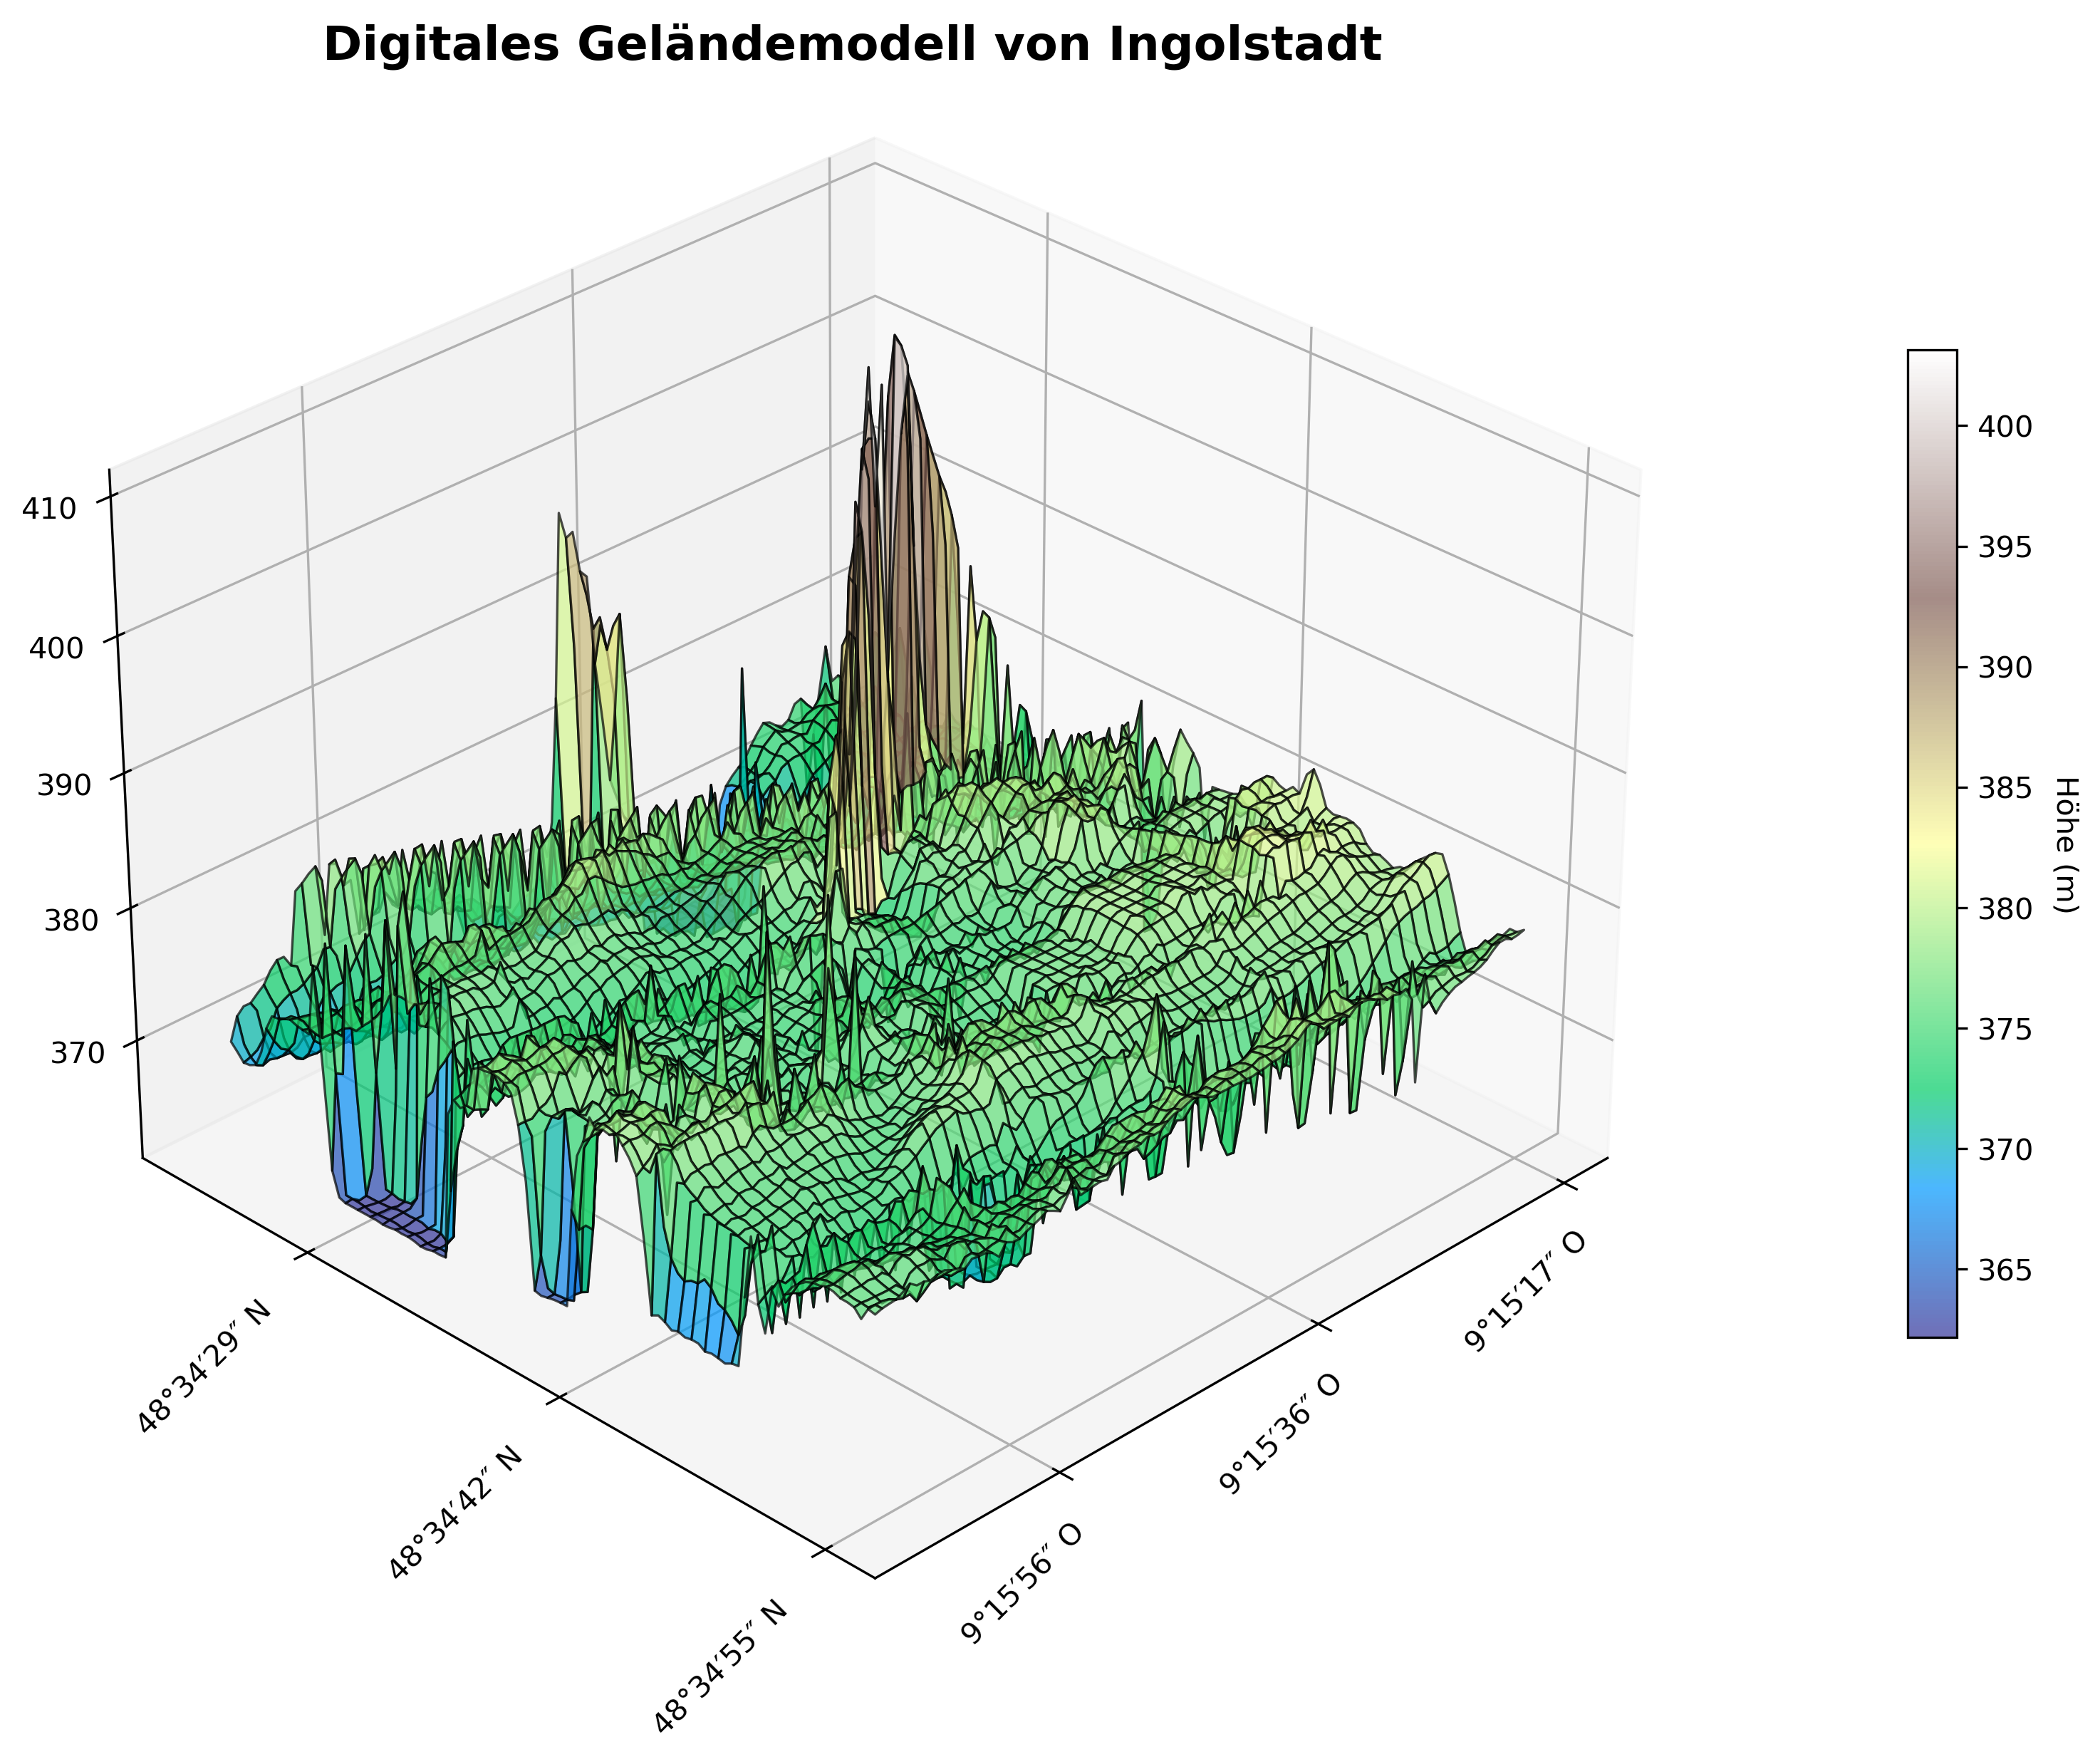
\includegraphics[width=0.8\textwidth]{figures/dgm_3d_wireframe_ingolstadt.png}
    \caption{Digital Geländemodell von Ingolstadt. Quelle: Eigene Darstellung}
    \label{fig:ingolstadt}
\end{figure}
\FloatBarrier
\subsection{Quadratmeterpreise}
Ein weiterer wichtiger Aspekt für ein realistisches Portfolio sind die Quadratmeterpreise. Die ungleiche Verteilung der Quadratmeterpreise ist allgemein bekannt. München gilt als die teuerste Stadt im Bundesland Bayern und in Deutschland und . Gemäß dem Bericht zum Immobilienmarkt liegen die Quadratmeterpreise für Eigenheime in der Stadt und im Landkreis München bei einem durchschnittlichen Preis von 10.200 EUR. In Kronach liegen die Preise bei 1.300 EUR \parencite{bayernlabo2024}. Es gibt große Varianz in den Preisen. Daher müssen die Darlehenspunkte an die jeweiligen Quadratmeterpreise des Standorts angeglichen werden. In Abbildung \ref{fig:preis} sind die Angebotspreise für Eigenheime in den bayerischen Landkreisen und kreisfreien Städten pro Quadratmeter in Euro dargestellt. Die Quadratmeterpreise für das Jahr 2023 wurden aufgeführt.
\begin{figure}[htbp]
    \centering
    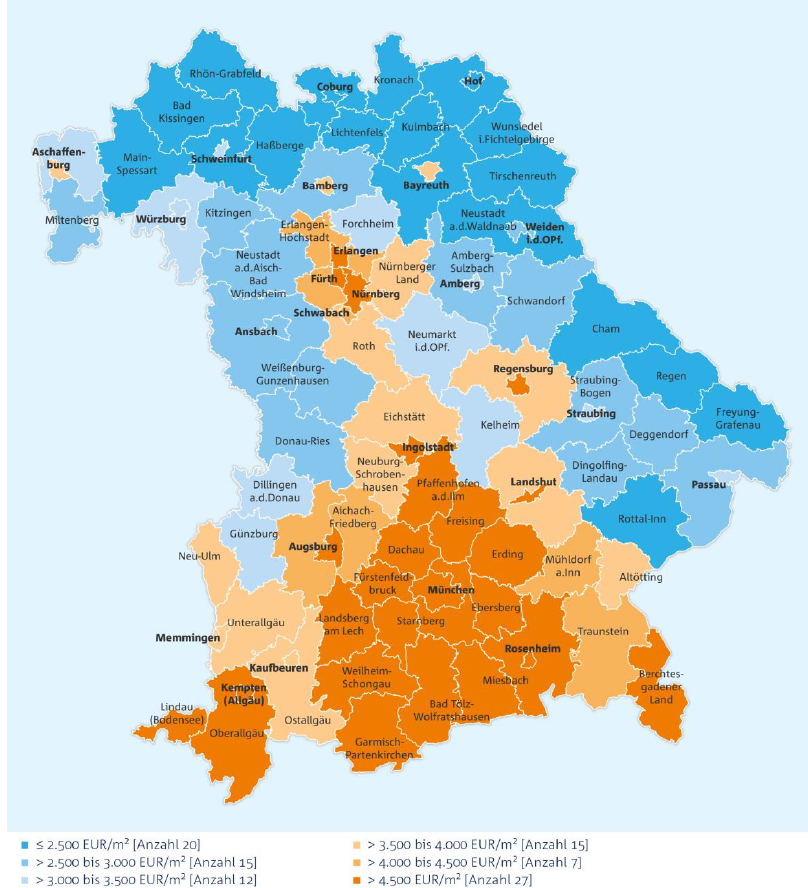
\includegraphics[width=0.8\textwidth]{figures/preism2.png}
    \caption{Angebotspreise 2023 in den bayerischen Landkreisen und kreisfreien Städten – Eigenheime – in €/m². Quelle: \textcite{bayernlabo2024} }
    \label{fig:preis}
\end{figure}
\FloatBarrier
\subsection{Verteilung der Energieeffizienzklassen in Bayern}
Wie bereits in Abschnitt \ref{sec:EPC} angegeben, haben Energieausweise für Wohngebäude einen direkten Einfluss auf die Betriebskosten und den Wert von Immobilien. Es gibt derzeit keine offiziellen Statistiken von staatlichen Behörden über die Verteilung von Energieeffizienzklassen in Bayern. Laut McMaker, einem führenden Maklerunternehmen in Deutschland, liegt Bayern jedoch an erster Stelle bei Wohnimmobilien mit positiven Energiekennwerten. In Bayern sind etwa 18\% der Wohnimmobilien energieeffizient (A+, A oder B), während 36\% schlechte Energiekennwerte haben \parencite{mcmakler2022}. Der Grund dafür liegt darin, dass die durchschnittliche Wohnimmobilie in Bayern erst 1991 gebaut wurde, was einen großen Unterschied im Vergleich zu anderen Bundesländern darstellt. Tabelle \ref{tab:epc_bayern} zeigt die Verteilung der Energieeffizienzklassen in Bayern.
\begin{table}[htbp]
    \centering
    \caption{Prozentuale Verteilung der Energieeffizienzklassen in Bayern}
    \label{tab:epc_bayern}
    \begin{tabularx}{\textwidth}{>{\raggedright\arraybackslash}X >{\centering\arraybackslash}X >{\centering\arraybackslash}X >{\centering\arraybackslash}X}
        \toprule
        & \textbf{A+, A, B} & \textbf{C, D, E} & \textbf{F, G, H} \\
        \midrule
        \textbf{Prozentanteil} & 18\% & 46\% & 36\% \\
        \bottomrule
    \end{tabularx}
\end{table}

Durch die Anwendung dieser Verteilung kann die \ac{EPC}-Verteilung in unser Hypothekenportfolio integriert werden, um eine möglichst realistische Darstellung des Portfolios zu erreichen.


\subsection{Ennergiepreise nach NGFS-Szenarien}\label{sec:ngfs_preis}
Die Auswertung der Heizenergiekosten imdeutschen Immobilienmark  stützt sich auf Daten aus den \ac{NGFS}-Szenarien und \textcite{imf2022}. Diese vorliegenden Daten bilden die Grundlage für die Prognose der Energiepreisentwicklung unter verschiedenen Klimaszenarien. Im Net Zero 2050 Szenario zeigen sich moderate Preissteigerungen für Öl, Gas und CO\textsubscript{2} Preis im nächsten Jahrzehnt. Ölpreise steigen aufgrund höherer Förderkosten, während Gaspreise schneller steigen, bedingt durch eine anhaltend starke Nachfrage. Die Preise für Emissionen dienen als wichtiger Indikator für das Transitionsrisiko. Es wird deutlich, dass höhere Emissionspreise mittelfristig nötig sind, insbesondere wenn Klimaschutzmaßnahmen verzögert umgesetzt werden.
Die Entwicklung der Preise für Öl, Gas und CO\textsubscript{2}-Emissionen nach \ac{NGFS}-Szenarien wird in Abbildung \ref{fig:ngfs_preis} visualisiert
\begin{figure}[htbp]
    \centering
    \begin{minipage}[b]{0.9\textwidth}
        \centering
        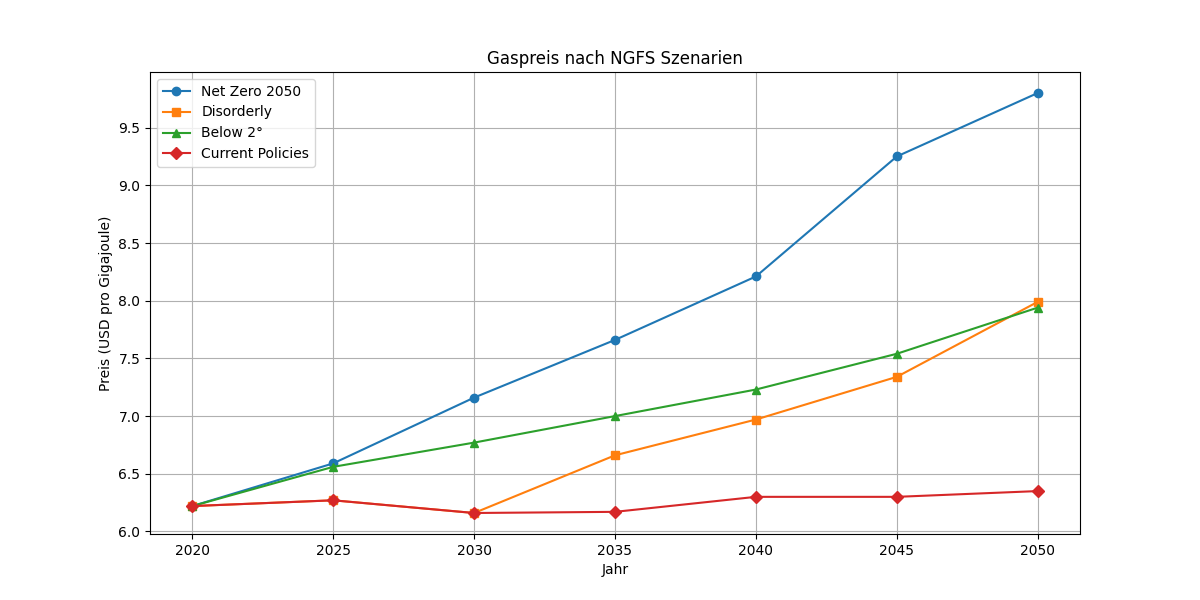
\includegraphics[width=\textwidth]{figures/gasprice.png}
    \end{minipage}
    \hfill
    \begin{minipage}[b]{0.9\textwidth}
        \centering
        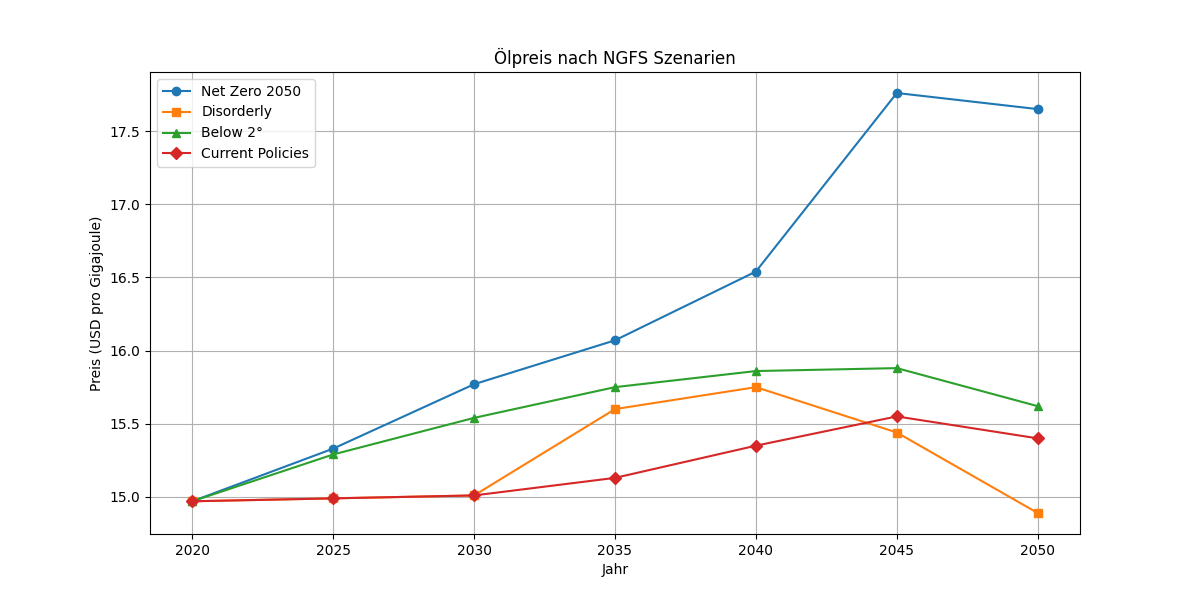
\includegraphics[width=\textwidth]{figures/Oilprice.png}
    \end{minipage}
    \hfill
    \begin{minipage}[b]{0.9\textwidth}
        \centering
        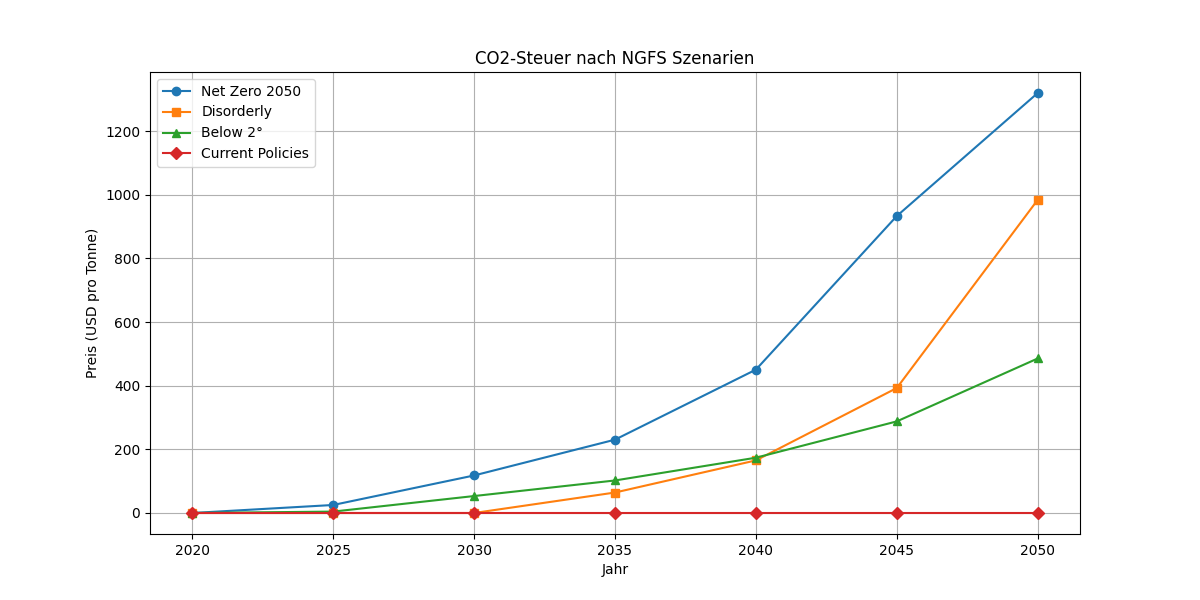
\includegraphics[width=\textwidth]{figures/co2price.png}
    \end{minipage}
    \caption{Energiepreise nach NGFS-Szenarien. Quelle: Eigeine Darstellung}
    \label{fig:ngfs_preis}
\end{figure}
\FloatBarrier



